\documentclass{article}
    % General document formatting
    \usepackage[margin=0.7in]{geometry}
    \usepackage[parfill]{parskip}
    \usepackage[utf8]{inputenc}
\usepackage[english]{babel}
\usepackage[nottoc]{tocbibind}
 \usepackage{hyperref}   
\usepackage{subcaption,graphicx}
    % Related to math
    \usepackage{amsmath,amssymb,amsfonts,amsthm}

\author{Tomas Musil}
\date{\today}
\title{Modular Robot Snake Training Environment and Reinforcement Learning of Simple Locomotion}

\begin{document}

\maketitle

\section{Background}
Reinforcement learning (RL) has widely been used for creating control policies for robots for a wide variety of tasks, such as locomotion of humanoid robots \cite{ppo}, spider-like robots \cite{emergence} or quadruped robots \cite{massively}.
In this project, I concerned myself with using RL algorithms to learn locomotion of a modular snake robot in various terrains.

The modular robot taught in simulation in this project is based on the hardware realization of a real modular snake robot, shown in Figure \ref{fig:hw}.
The robot system was constructed by me and my 3 other colleagues at the Czech Technical University and features very affordable parts, open-source design and simple communication and software stack.
% It is also a reason for me taking this course, where I intended to learn more about RL and apply it to creating a RL-based controller for this robot system.

RL is particularly of interest for complicated robots for which it is hard to create a controller by hand. 
As such, I believe RL to be well suited for developing controllers for this particular robotic system, since it is physically capable of for example climbing up stairs, but I see no way of designing a controller for that without RL.
Furthermore, it would be difficult to construct a controller every time the user wants to change the robot configuration, and having automatic controller generation could be very useful.

\begin{figure}[!h]
 \centering 
  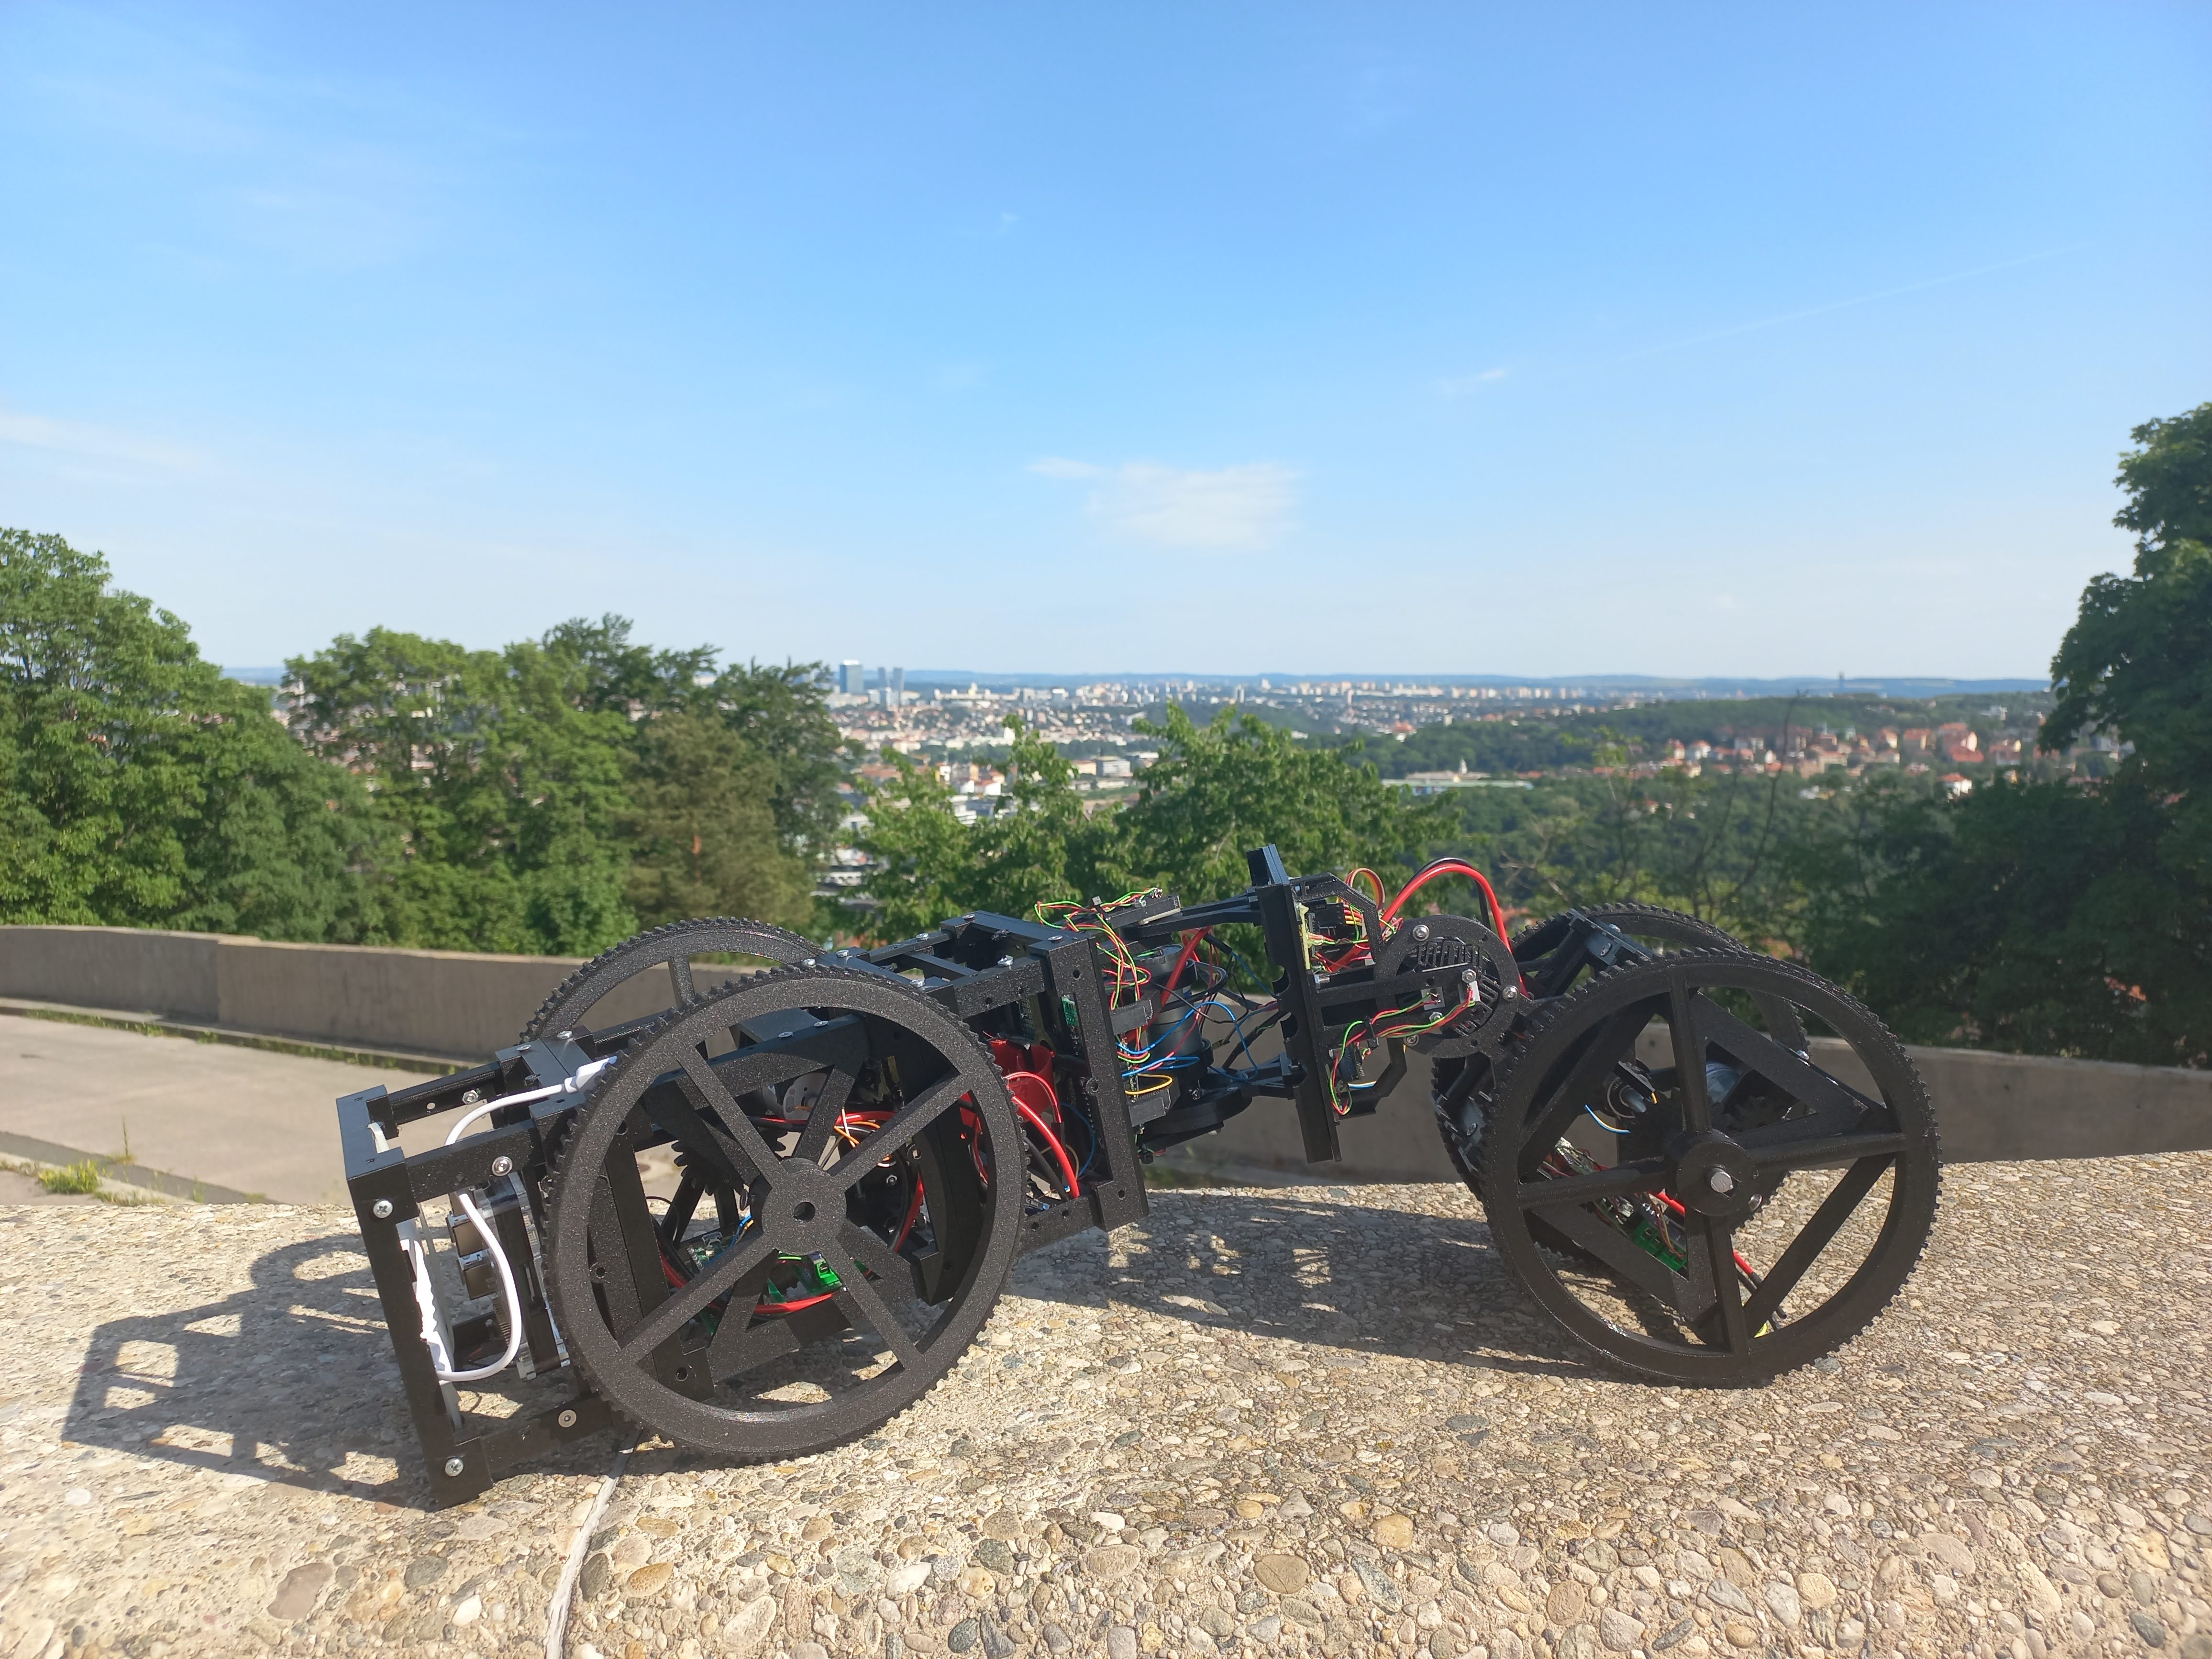
\includegraphics[width=.8\textwidth, trim={15cm 10cm 10cm 45cm}, clip]{fig/snek_real.jpg}
  \caption{The real hardware of the modular robot system for which I constructed the simulation in this project, in configuration with a head module followed by a wheel module, two servo modules to allow bending up and down and steering, and one more wheel module}
\label{fig:hw}
\end{figure}

\section{Problem Definition}
The goal of this project is to:
\begin{itemize}
    \item Construct a custom gym environment which would allow effortless definition and spawning of different configuration of the modular robot which could be transferred to the real robot, and have multiple terrains on which to learn movement.
    % \item Train moving in one type of terrain for multiple robot configurations to see how the number of degrees of freedom of observation and actions affect the training.
    \item Train on two types of terrain using two different RL algorithms. First a simple uneven terrain simulating for example the floor of a forest.
      Secondly on an environment with stairs.
\end{itemize}

\section{Methods}
\subsection{Custom AI Gym Environment Construction}
For the purpose of this project, I developed a custom AI gym environment from scratch. Here is the main description of the developed environment:
\begin{itemize}
  \item \textbf{General features:} The environment uses the PyBullet physics engine for its physics simulation. 
The environment constructor takes as input the desired configuration of modules in the robot (specified by a string of tuples (module type, module orientation w.r.t. the previous module) and creates an URDF file which it uses to spawn the snake robot.
Furthermore, the environment currently supports 2 different terrains on which the robot can learn to move.
    I created 2 terrains using the open-source software Blender and these terrains are shown in Figure \ref{fig:terrains}. The terrain \textit{bumps} is randomly rotated around the $z$ axis on every reset to simulate random bumpy terrain for the robot.
    The number of actions and observation naturally depends on the number of servo modules $n_{servo}$ and wheel modules $n_{drive}$.
  \item \textbf{Observations:} The environment has $3+ n_{servo}$ continuous observations. These are an ensemble of roll, pitch, yaw of the robot (simulating measurements from an affordable IMU sensor, although without noise), and the current angle of every servo module in the robot.
  \item \textbf{Actions:}  The environment has $n_{servo} + n_{drive}$ actions, with each servo having a position reference input (not velocities), and each drive module having a velocity reference input. The position and velocity control is done by pybullet for the robot joints.
    Additionally, the physics simulation does 5 steps for every environment step (=for every action) to simulate a low control bandwidth, which is present in the real-world robot, and to make the movements less jittery.
  \item \textbf{Reward:} The reward differs for the 2 terrain types. For teaching to move forward (in $x$ direction) on bumpy terrain, the robot gets a reward $r_{bumps} = 100*dx - 50*|dy|$ every timestep. For moving on stairs, the robot is motivated to lift its head to climb the stairs by adding a reward for moving in the $z$ direction, so its reward is $r_{stairs} = 100*dx - 50*|dy| + 200*dz$.
    I experimented with adding a penalty for rotation along the $z$ axis to force the robot to move forward more quickly, but this proved to be counter productive.
    Additionally, in both terrains, the agent gets a large fixed reward if it reaches the end of the terrain in the $x$ direction.
  \item \textbf{Reality gap:} The masses and moments of inertia of robot links, max speed of wheels and max force and speed of the servo modules were just approximately estimated. Also the real-world servos feature a spring for SEA actuation, which is not modeled in the simulation servos.
    Therefore, this simulation is more of a proof of concept and would need additional work to be deployable 1:1 on the real hardware.
    This would require a lot of additional work in the form of a larger project.
\end{itemize}

\begin{figure}[ht]
\begin{subfigure}{.5\textwidth}
  \centering
  % include first image
  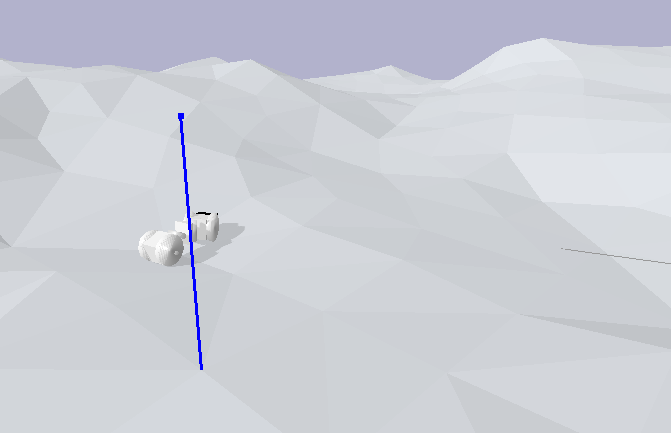
\includegraphics[width=.95\linewidth]{fig/bumps.png}  
  \caption{The terrain type - \textit{bumps}}
  \label{fig:sub-first}
\end{subfigure}
\begin{subfigure}{.5\textwidth}
  \centering
  % include second image
  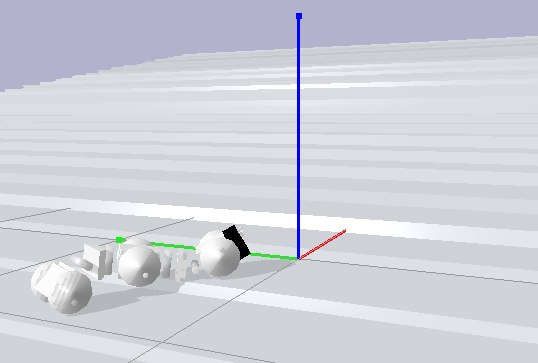
\includegraphics[width=.95\linewidth]{fig/stairs.png}  
  \caption{The terrain type - \textit{stairs}}
  \label{fig:sub-second}
\end{subfigure}
  \caption{The two learning scenarios. 
  A configuration with 2 wheel modules and 2 servos is used for the \textit{bumps} terrain and a longer robot configuration with 3 wheel modules and 4 servos is used for the \textit{stairs} terrain.
  The \textit{bumps} terrain is also randomly rotated around the vertical axis at every reset. }
\label{fig:terrains}
\end{figure}

\subsection{Training Methods}
% First, I experimented with the algorithms from the library and found PPO \cite{ppo} to work the best, A2C to work slightly for the bumpy terrain but not for stairs, and the other algorithms were not learning anything meaningful for the constructed environment.
% For training in both tasks, I decided to use the library TODO.
% Therefore, in this paper I showcase 2 experiments.
For training the robot on the 2 terrain types, I used the open-source library stable-baselines3 \cite{stable-baselines3}, which allows easy implementation of RL algorithms such as A2C, PPO, DDPG, etc.
I experimented for some time with various algorithms, and found PPO and A2C to work best for this environment, which is why I chose them for the demonstration experiments.
Both are using a Multi-Layer Perceptron (MLP) policy in all cases.

The first experiment I designed was comparing A2C and PPO on the same setup of the \textit{bumpy terrain} scenario.
I used the default hyperparameters and the train() function from stable-baselines3 and trained for 100 episodes of 3000 steps each.

Second experiment was learning to go up in the \textit{stairs} scenario. 
% I found that out of the algorithms with default hyperparameters, only PPO was able to learn to go up the stairs, and therefore only showcase PPO. 
I also used the train() function from stable-baselines3 and trained for 300 episodes of 3000 steps each.
% I used the default hyperparameters and the train() function from stable-baselines3 and trained for 200 episodes of 3000 timesteps each.

\section{Results}
% First round - stairs, long, 2 different algos (2g)
% Second round - bumps, 1 algo, 2 different configurations (2g)
% 3rd round - bumps, 2 algo, 2 different configurations (4g)
The results of learning on \textit{bumpy terrain} can be seen in Figure \ref{fig:bumps}.
In this experiment, PPO was learning more slowly than A2C, but A2C was somewhat inconsistent in the episode rewards, while PPO was steadily increasing the episode reward.
Both methods learned fast compared to the \textit{stairs} terrain, which is understandable, since this task is substantially easier.
% PPO learned a policy much faster than A2C and TODO.

The results of learning on \textit{stairs} using PPO can be seen in Figure \ref{fig:stairs}.
In this experiment, PPO was able to gradually learn a stair climbing motion.
% This motion was 
% , while A2C was unable to produce a policy that would get it over the first step, which can be seen by the quick stagnating in the graph.
A2C was able to not fall off the back side of the terrain, and slowly got better at not going backwards, but was unable unable to get over even the first step, which corresponds to the plaetau in the graph.
A2C, in essence, learned not to fall down the stairs, but could not climb forward, whereas PPO managed to climb the stairs and even get to the end of the stairs (this corresponds to the high reward outliers near the end).
 
I have also published a video of the PPO agent after 300 episodes here: \href{https://www.youtube.com/watch?v=A939OQfjrN8}{https://www.youtube.com/watch?v=A939OQfjrN8}

\begin{figure}[ht]
\begin{subfigure}{.5\textwidth}
  \centering
  % include first image
  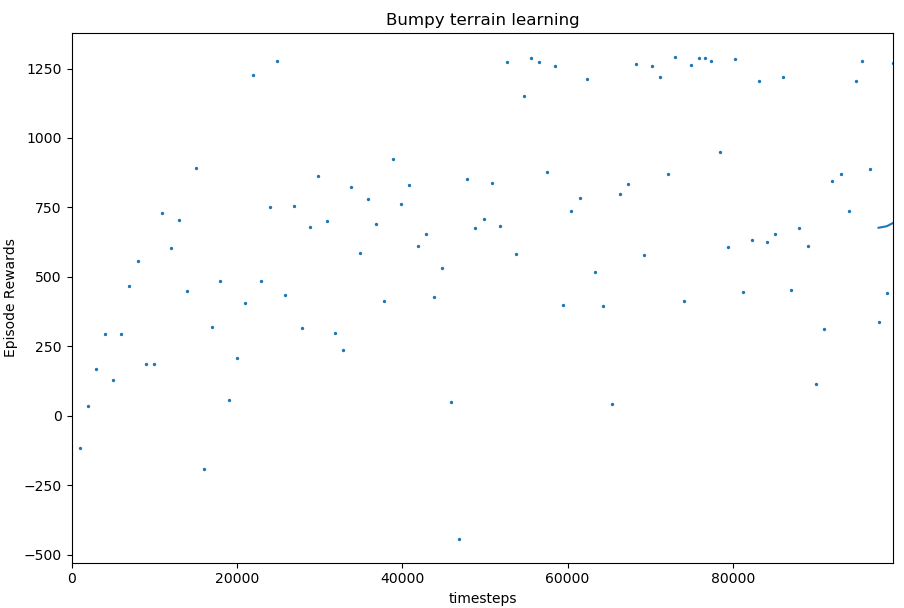
\includegraphics[width=.95\linewidth]{figc/Bumpy_terrain_learning_100ep_a2c.png}  
  \caption{A2C}
  \label{fig:sub-first}
\end{subfigure}
\begin{subfigure}{.5\textwidth}
  \centering
  % include second image
  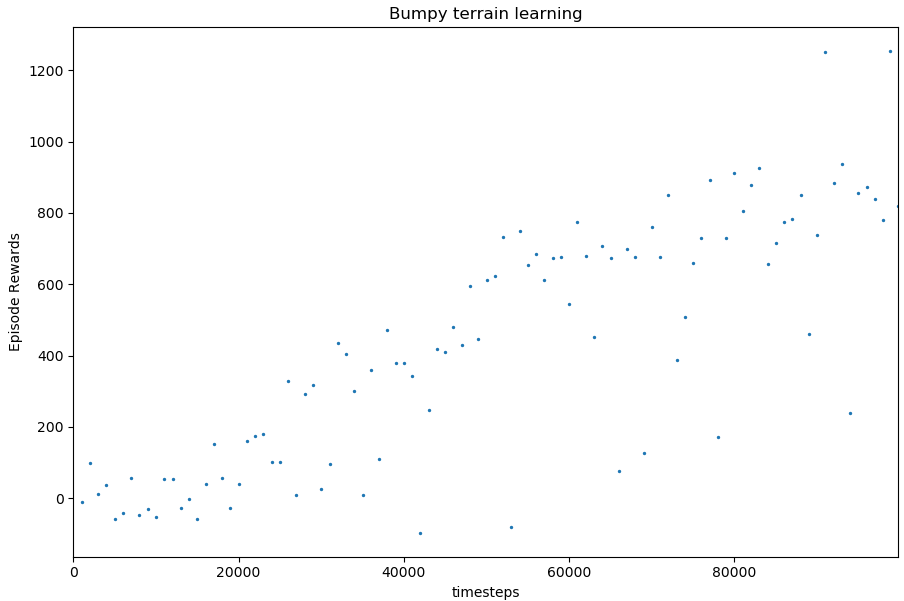
\includegraphics[width=.95\linewidth]{figc/Bumpy_terrain_learning_100ep_ppo.png}  
  \caption{PPO}
  \label{fig:sub-second}
\end{subfigure}
  \caption{Results from learning PPO and A2C models on the \textit{bumps} terrain for 100 episodes.}
\label{fig:bumps}
\end{figure}

\begin{figure}[ht]
\begin{subfigure}{.5\textwidth}
  \centering
  % include first image
  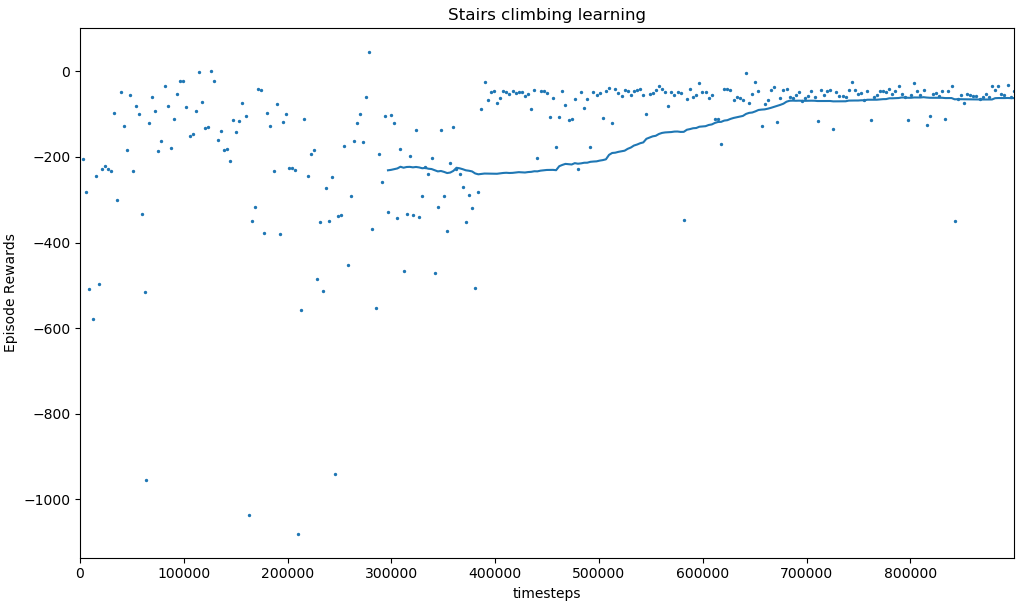
\includegraphics[width=.95\linewidth]{figc/Stairs_climbing_learning_300ep_final_a2c.png}  
  \caption{A2C}
  \label{fig:sub-first}
\end{subfigure}
\begin{subfigure}{.5\textwidth}
  \centering
  % include second image
  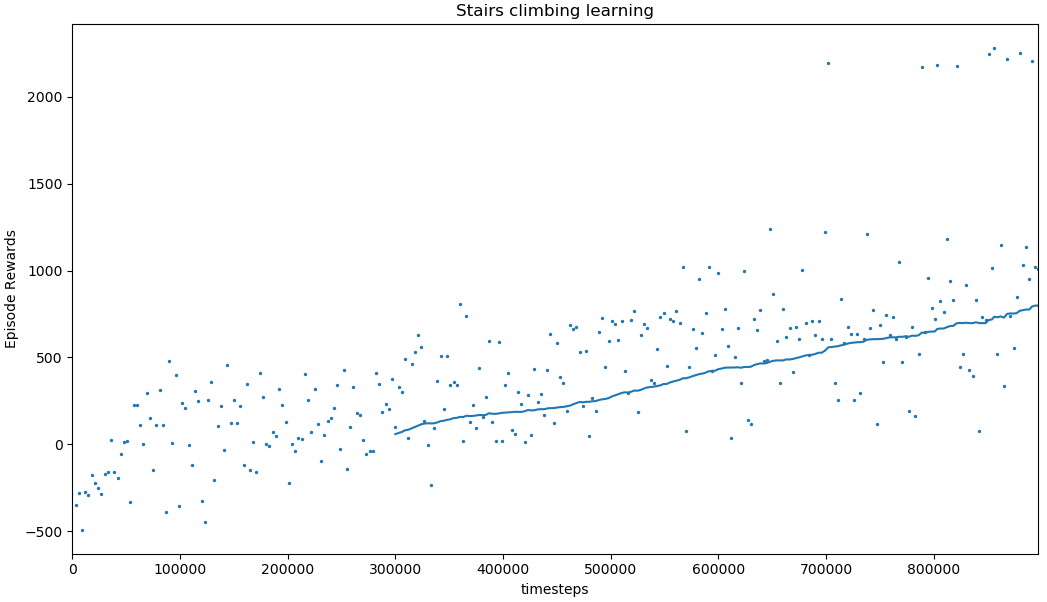
\includegraphics[width=.95\linewidth]{figc/Stairs_climbing_learning_300ep_final.png}  
  \caption{PPO}
  \label{fig:sub-second}
\end{subfigure}
\caption{Results from learning PPO and A2C models on the \textit{stairs} terrain for 300 episodes.}
\label{fig:stairs}
\end{figure}
\section{Discussion}
I believe it is a great success that I managed to construct a working gym environment and implement the PPO algorithm for it and succesfully make the model learn a motion that can climb the stairs.

An interesting thing is why PPO learned more slowly than A2C in the \textit{bumps} terrain.
From observing the two learning processess in the PyBullet GUI, it seemed to me that A2C does not produce such noisy action signals as PPO, meaning that PPO in the stable-baselines3 likely uses some action noise, while A2C does not.
Due to time constraints, I could not have investigated this further.

Another notable thing is that, as can be seen in the video in the Results section showing the PPO model scale stairs, the robot in that case produces a sort of "oscillatory" motion where it throws its body from side to side.
I was worried if a simple MLP-policy would be sufficient to learn stair climbing and if it did not rather need a recurrent policy, as the robot would need to develop some "gait" which would need some recurrence to move up stairs.
However, it seems to me that thanks to the complexity of the body of the robot, and since all joints of the servos are controlled AND observed, and multiple physics steps are happening between each environment step, the robot was able to form this kind of gait without any recurrence in the model itself.
My explanation for this is that the MLP-policy model likely learned a gait such as (body bent left $=>$ bend body right and up, body bent right $=>$ bend body left and down).
The possible fact that the learning solved the recurrence problem in this way is fascinating.

There are many ways this project can be built upon.
Firstly, I would like to work more closely with the real hardware and try running the learned policy on a real robot, and then seeing the discrepancies and working on bridging the reality gap as much as possible. 
Additionally, I would like to, in the future, add some form of touch/force perception in a physically realizable manner, for example using tiny bumpers/buttons in the front of the robot or on the servo module, or also measuring the current and velocity of the wheels to infer if they are touching ground or not.
I believe that would make the robot learn to climb stairs/rocks even better.

% Mention - happy that I was able to make it learn on the stairs and on the bumps.
% Fun would be putting it on real HW and testing its movement and trying to bridge the reality gap (different masses, powers of motors, delays, springiness, ...) which would take a lot of effort, maybe for one full masters thesis.


% \bibliographystyle{IEEEtran}
\bibliographystyle{unsrt}
% DO NOT ERASE THE NEXT LINE,
% ONLY COMMENT IT AND DECOMMENT THE NEXT-NEXT, IF YOU NEED
% if you need it, get the repo git://redmine.laas.fr/laas/users/afranchi/bib.git and configure your bibinput in order to have : bibAlias,bibMain,bibNew,bibAF
% \bibliography{main.bib}
\bibliography{main.bib}

\end{document}
